%Einfache Vorlage fÅžr eine mit Latex realisierte Hausarbeit von http://www.studieren-info.de
%Du kannst diese Vorlage fÅžr deine Hausarbeit beliebig anpassen%


%-------------------
%Beginn des Kopfbereiches
%-------------------

%Wir verwenden eine DIN-A4-Seite und die Schriftgrš§e 12.
\documentclass[a4paper,12pt]{scrartcl} 


%Diese drei Pakete benštigen wir fŞr die Umlaute, Deutsche Silbentrennung etc.
%Apple-Nutzer sollten anstelle von \usepackage[latin1]{inputenc} das Paket \usepackage[applemac]{inputenc} verwenden
\usepackage[utf8]{inputenc}
\usepackage[ngerman]{babel}
\usepackage[T1]{fontenc}

% Numerierte Liste
\usepackage{enumitem} 

%Grafikpaket
\usepackage{graphicx}

%Syntax Highlighting
\usepackage{listings}

%Text um Bild fließen lassen
\usepackage{wrapfig} 

%Subsubsubsection alternative
\usepackage[outermarks]{titlesec}
\titleformat{\section}
  {\normalfont\Large\bfseries}{\thesection}{1em}{}
\titleformat{\subsection}
  {\normalfont\large\bfseries}{\thesubsection}{1em}{}
\titleformat{\subsubsection}
  {\normalfont\normalsize\bfseries}{\thesubsubsection}{1em}{}
\titleformat{\paragraph}
  {\normalfont\normalsize\bfseries}{\theparagraph}{1em}{}
\titleformat{\subparagraph}
  {\normalfont\normalsize\bfseries}{\thesubparagraph}{1em}{}

\titlespacing*{\section}      {0pt}{3.5ex plus 1ex minus .2ex} {2.3ex plus .2ex}
\titlespacing*{\subsection}   {0pt}{3.25ex plus 1ex minus .2ex}{1.5ex plus .2ex}
\titlespacing*{\subsubsection}{0pt}{3.25ex plus 1ex minus .2ex}{1.5ex plus .2ex}
\titlespacing*{\paragraph}    {0pt}{3.25ex plus 1ex minus .2ex}{1.5ex plus .2ex}
\titlespacing*{\subparagraph} {0pt}{3.25ex plus 1ex minus .2ex}{1.5ex plus .2ex}

% Farben definieren
\usepackage{xcolor}
\definecolor{codeGray}{RGB}{240,240,240}
\definecolor{codeBlack}{RGB}{0,0,0}
\definecolor{codeRed}{RGB}{221,0,0}
\definecolor{codeBlue}{rgb}{0,0,187}
\definecolor{codeYellow}{RGB}{255,128,0}
\definecolor{codeGreen}{RGB}{0,119,0}

% 
 und zuweisen
\lstset{%
    language=PHP,%
    %
    % Farben, diktengleiche Schrift
    backgroundcolor={\color{codeGray}},% 
    basicstyle={\scriptsize\ttfamily\color{codeGreen}},% 
    commentstyle={\color{codeYellow}},%
    keywordstyle={\color{codeBlue}},%
    stringstyle={\color{codeRed}},%
    identifierstyle={\color{codeBlue}},%
    %
    % ZeilenumbrÃŒche aktivieren, Leerzeichen nicht hervorheben
    breaklines=true,%
    showstringspaces=false,%
    % 
    % Listing-Caption unterhalb (bottom)
    captionpos=b,%
    % 
    % Listing einrahmen
    frame=single,%
    rulecolor={\color{codeBlack}},%
}

%Das Paket erzeugt ein anklickbares Verzeichnis in der PDF-Datei.
\usepackage{hyperref}

%Das Paket wird fÌr die anderthalb-zeiligen Zeilenabstand benštigt
\usepackage{setspace}

%EinrÃŒckung eines neuen Absatzes
\setlength{\parindent}{0em}

%Definition der Rander
\usepackage[paper=a4paper,left=30mm,right=30mm,top=30mm,bottom=30mm]{geometry} 

%Abstand der Fu§noten
\deffootnote{1em}{1em}{\textsuperscript{\thefootnotemark\ }}

%Regeln, bis zu welcher Tiefe (section,subsection,subsubsection) Überschriften angezeigt werden sollen (Anzeige der †berschriften im Verzeichnis / Anzeige der Nummerierung)
\setcounter{tocdepth}{5}
\setcounter{secnumdepth}{5}

%-------------------
%Ende des Kopfbereiches
%-------------------




%-------------------
%Hier beginnt der Text deiner Hausarbeit
%-------------------
\begin{document}


%Beginn der Titelseite
\begin{titlepage}
\begin{small}
\vfill {
\begin{wrapfigure}{r}{0.4\textwidth}
 \vspace{-16pt}
 \centering 
 
\includegraphics[width=0.35\textwidth]{Bilder/hs_logo.png}
 \vspace{-10pt}
\end{wrapfigure}
Hochschule Kaiserslautern\\ 
Entwicklung verteilter Anwendungen in Java\\ 
Sommersemester 2015}
\end{small}


\begin{center}
\begin{Large}
\vfill { \textsf{\textbf{
Chat-Applikation auf Server- und Clientebene
}}}
\end{Large}
\end{center}

\begin{small}
\vfill 868407 \\ Dorian Weidler, Luca Hartmuth, Julian Meisel \\
\today
\end{small}

\end{titlepage}
%Ende der Titelseite


%Inhaltsverzeichnis (aktualisiert sich erst nach dem zweiten Setzen)
\tableofcontents
\thispagestyle{empty}

%Beginn einer neuen Seite
\clearpage

%Anderthalbzeiliger Zeilenabstand ab hier
\onehalfspacing

\pagestyle{plain}


\section{Einleitung}
Ziel des Server-Teilprojekts war es einen Multiuser-Chat-Server zu entwickeln, der fehlerfrei Verbindungen mit mehreren Nutzern aufbaut, diese verwaltet und sie auch wieder abbaut.\\

Eine weitere Anforderung war den Server so parallel zu gestalten wie möglich aber trotzdem so performant wie möglich zu halten. Resultat war, dass jedem User ein Thread zusteht, der beim Verbinden für ihn geöffnet wird und ein Thread, der nur für seine Heartbeats geöffnet wird. Im ersten Thread werden all seine Aktionen (Login, Registration und Nachrichten, damit verbunden auch Befehle) abgearbeitet.\\

Des Weiteren haben wir die persönliche Anforderung an das Client Teilprojekt gestellt, dass möglichst wenige Updates für den Endnutzer bereitgestellt werden müssen. Aus diesem Grund haben wir uns für eine rudimentäre GUI entschieden, die ein großes Textfeld für die empfangen und ein kleines Textfeld für die zu sendenden Nachrichten enthält. Außerdem befinden sich noch ein kleines Label auf dem GUI, das anzeigt in welchem Channel man sich befindet und eine Userliste mit den aktuell im Channel befindlichen Usern.\\

Alle weiteren Aktionen, wie zum Beispiel das Ändern des aktuellen Channels, werden mittels Kommandos im Chat abgearbeitet. So sieht zum Beispiel der Befehl zum Ändern des aktuellen Channel wie folgt aus:
\begin{lstlisting}[frame=single,caption=Beispiel eines Befehls]
/join #channelname
\end{lstlisting}
Wir sahen darin einen mächtigen Vorteil, und zwar hat unserer Meinung nach der Serveradministrator mehr Kenntnisse bzgl. seines Computers als der Endanwender. Ihm sollte man die Updates zumuten können. Des Weiteren stellt sich das Verteilen der Updates auf eine Schar von Usern als deutlich schwerer heraus als des reine Verteilen auf die Server. Außerdem muss der Fall, dass ein Nutzer mit einer älteren Version mitchatten möchte, in aller Regel nicht beachtet werden. Sollte der Client doch einmal geupdated werden müssen, so muss dieser Fall natürlich gründlichst geprüft werden und ggf. durch weitere Änderungen im Serverquelltext ebenfalls abgedeckt werden.\\

In unserem aktuellen Bestreben ist das Updaten des Funktionsumfangs eine eher einseitige Angelegenheit für den Anbieter des Dienstes und damit auch seine/n Administrator/en, die vermutlich ein größeres technisches Verständnis haben als ein Benutzer.
\section{Serverdokumentation}
\subsection{Klassenerklärungen}
\begin{itemize}
\item CMain: Das ist die Einstiegsklasse des Programms, sie liest mithilfe von CConfigParser die Konfigurationsdatei aus und gibt die nötigen Einstellungen an den Konstruktor der CServer Klasse weiter um ein solches Objekt zu erzeugen.
\item CServer: Diese Klasse erbt von Thread und bekommt als Parameter im Konstruktor den Standard-Channelnamen und den Port auf dem der Chatserver horchen soll. Danach wird der Thread gestartet, indem ein Serversocket auf dem, in der Konfigurationsdatei angegebenen, Port öffnet, alle Channels aus der channels.lst mittels des CChannelParsers ausliest und auf eingehende Verbindungen wartet. Bei einer neuen Verbindung wird ein CClientHandler Objekt erzeugt und der Client zu den verbundenen Clients hinzugefügt. Daraufhin wartet der Server wieder auf neue Verbindungen.
\item CClientHandler: Diese Klasse erbt ebenfalls von Thread. Im Konstruktor werden zunächst alle programmierten Befehle jeweils als CCommand Objekte angelegt, die den Befehl selbst und einen dazugehörigen Hilfetext beinhalten. Dann wird dem geöffnet Socket, d.h. der Verbindung zum Client, ein Timeout gesetzt, der dazu dient eine Exception zu werfen, wenn der Timeout ausläuft. Die Exception wird abgefangen und dabei geprüft ob die Verbindung noch besteht. Ist dem so, wird die Verbindung zum Client geschlossen und alle anderen Clients dementsprechend informiert. Der ClientHandler startet sich dann selbst als Thread und liest aus dem InputBuffer jeweils 256 Byte und prüft diese auf die Packet-Struktur. Stimmt sie wird das Paket entsprechend auf die nötige Länge beschnitten und ein CClientPacket Objekt damit erzeugt und darauf die handlePacket-Methode des Objekts aufgerufen. Dann liest er wieder aus.
\item CClientPacket: Diese Klasse dient dazu, ein Packet zu prüfen, in seine Einzelteile zu zerlegen und dann entsprechend seines Typs zu behandeln. Zunächst werden dem Konstruktor das gesamte Packet als String, der aufrufende CClientHandler und die IP des verbundenen Clients. Aus dem gesamten Paket wird dann der Typ ausgelesen und als Objektattribut gesetzt. In der handlePacket()-Methode wird nun anhand des Typs geprüft was getan werden muss bzw. ob etwas getan werden muss. (Wird z.B. ein Login- oder Registerpacket von einem eingeloggten Client empfangen, wird dieses verworfen) In den entsprechenden Methoden processRegisterOrLoginPacket() (Behandelt beides, bekommt aber als Parameter ob es ein Login- oder Registerpacket ist, weil der Anfang gleich ist. Am Ende wird nur unterschieden ob ein Login gemacht werden muss oder eine Registration) oder processMessage() werden die Pakete dann entgültig zerlegt und ihre Einzelteile ausgewertet.
\item CHeartbeat: Erbt von Thread und beinhaltet eine Schleife, die so lange immer wieder durchlaufen wird, wie ein Heartbeat empfangen wird. Ein Heartbeat ist eine jede Aktion des Clients (explizite Heartbeats, Nachrichten, Kommandos, ...). Bei einer Aktion wird von der bearbeitenden Klasse die beatReceived()-Methode des zugehörigen CHeartbeat-Objekts aufgerufen, was den aktuellen Heartbeat-Empfangen-Status auf "true" setzt.
\item CClient: Dient als Repräsentation des Clients auf dem Server. Diese Klasse dient eigentlich nur als Datenhalter. Die einzige richtige Methode der Klasse ist die setCurrentChannel()-Methode, die den Channel wächselt, dem Client ein entsprechendes MessagePaket schickt mit allen im neuen Channel befindlichen Clients und ruft die leaveChannel Methode beim aktuellen Channel für den Client auf und die joinChannel Methode beim neuen Channel.
\item CChannel: Dient als Repräsentation eines Channels und bietet die Methoden joinChannel und leaveChannel die jeweils die Clients über neue User im Channel bzw. verlassende User informiert.
\item CChannelParser: Liest die channels.lst aus und gibt ein Array aller Channels aus.
\item CConfigParser: Liest die config.cfg aus und speichert die darin befindlichen Informationen als Objektattribute des Parsers. Diese können mittels der Getter Methoden ausgelesen werden.
\item CServerPacket: Dient als Bauplan für Pakete die vom Server zu einem Client gesendet werden. Darin ist auch die sendMessage Methode, die einen Empfänger und einen Sender als Attribut bekommt. So können z.B. Private Nachrichten realisiert werden. Um eine Nachricht an alle zu schicken müsste einfach durch alle verbundenen Clients iteriert werden. Nur für Nachrichten ist weiteres außer dem Packetheader nötig. Alle anderen Pakete (Server -> Client) bestehen nur aus dem Packetheader.\\
Mehr dazu erfahren Sie im Packet Structure Abschnitt.
\item CServerPacketHeaders: Beinhaltet nur eine Methode um den Packetheader eines Serverpackets auf Gültigkeit zu prüfen.
\item CLogger: Ist eine Hilfsklasse im in die angegebene Datei zu schreiben. Wird zum Beispiel in der utils Klasse benutzt um die Servernachrichten in die log.txt Datei zu schreiben.
\item utils: Beinhaltet die Ausgabemethoden debugMsg, errorMsg und infoMsg und eine isNumber Methode um zu prüfen ob es sich bei einem String um eine valide Zahl handelt oder nicht. Die Ausgabemethode debugMsg() prüft dabei zunächst ob der Server aktuell im Debugmodus ausgeführt wird. Ist dem nicht der Fall, wird keine Ausgabe getätigt.
\item Exceptions-Package: Enthält alle Exceptions.
\end{itemize}

\subsection{Installation}
Zur Installation muss lediglich das .zip Verzeichnis mit einem entsprechenden Programm entpackt werden und daraufhin die config.cfg nach eigenem Ermessen bearbeitet werden.
\begin{lstlisting}[frame=single,caption=Beispielinhalt der Konfigurationsdatei]
/join #channelnamePort = 1337
QueueLength = 1500
DefaultChannel = #default
\end{lstlisting}
Daraufhin muss noch die channels.lst bearbeitet werden. \textbf{Wichtig:} Der DefaultChannel aus der config.cfg \textbf{muss} dort nochmal stehen! Eine Zeile pro Channel!
\begin{lstlisting}[frame=single,caption=Beispielinhalt der Channeldatei]
#default
#test
\end{lstlisting}

Damit ist die Grundkonfiguration des Servers abgeschlossen und der Server kann mit dem nachfolgenden Befehl in Betrieb genommen werden:
\begin{lstlisting}[frame=single,caption=Startbefehl]
java -jar Server.jar
\end{lstlisting}
Optional kann diesem Befehl noch ein \textbf{true} folgen, damit werden Debug Meldungen ausgegeben, dies sollte aber aufgrund der Übersichtlichkeit nur zu Testzwecken und nur von einem Entwickler aktiviert werden.

\subsection{Hinzufügen eines neuen Befehls}
Dazu muss die onMessageReceived()-Methode entsprechend modifiziert werden. Dort sind bereits einige Befehle angelegt, die essentiell für die Funktionalität sind.\\

Hier noch ein weiteres Beispiel, dass Sie theoretisch Copy\&Paste integrieren können.
\begin{lstlisting}[frame=single,caption=Beispielinhalt der Channeldatei]
		// Bei onMessageReceived in die If-Abfrage integrieren
 		else if(message.startsWith("/test")){
			/* Fall: /test als Beispiel */
			sendMessage("Testnachricht", mServer.getServerClient());			
		}
		/* Im Konstruktor den anderen registerCommand anhaengen. */
		registerCommand("/test", "Dient als Beispiel."); 
\end{lstlisting}
Im Beispiel wird ein Befehl "/test" {eingefügt}, der dem User nur eine Nachricht "Testnachricht" mit dem Serverclient schickt.
\clearpage

\section{Clientdokumentation}
\subsection{Klassenerklärungen}
\subsubsection{Exceptions-Package}
Enthält, wie der Name vermuten lässt, alle Exceptions.

\subsubsection{Functions-Package}
\begin{itemize}
\item CHeartbeat: Diese Klasse ist analog zu der Serverklasse. Sie startet eine Schleife, die prüft ob der aktuelle Heartbeat erhalten wurde oder nicht. Eine Methode beatReceived() setzt dazu eine boolesche Variable auf "true".
\item CLoginListener: Ist ein ActionListener, der dann aufgerufen wird, wenn der Benutzer auf der wndLogin-Oberfläche auf den Login Knopf drückt. Bei diesem Aufruf wird ein Login-Packet konstruiert und an den Server gesendet mit den Daten aus den Username und Passwort Textboxen.
\item CPacketListener: Diese Klasse stellt einen Thread da, der bei erfolgreichem Login gestartet wird. Zum Design dieser Klasse wurde das Singleton-Pattern genutzt, da von dieser Klasse nur ein Objekt benötigt wird und erstellt werden soll. In diesem Objekt werden eingehende Packets eingelesen und verarbeitet.
\item CRegisterListener: Ist ein ActionListener, der dann aufgerufen wird, wenn der Benutzer sich mittels der wndRegister-Oberfläche auf dem Server registriert. Daraufhin sendet der Client ein Registerpacket, das mit den angegebenen Daten aufgebaut wurde.
\item CSendMessageListener: Ist ein ActionListener, der von der wndChat-Oberfläche aufgerufen wird wenn der Benutzer eine Nachricht absendet. Sie baut ein Message Packet auf, mit dem Payload und der dazugehörigen Länge.
\end{itemize}

\subsubsection{GUI-Package}
\begin{itemize}
\item wndChat: Diese Klasse stellt das Hauptfenster des Chats dar.\\
\begin{minipage}{\linewidth}
            \centering
            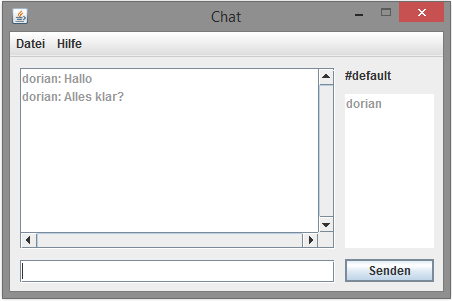
\includegraphics{Bilder/main_client.png}
            \captionof{figure}{wndChat-Oberfläche}
\end{minipage}

\item wndLogin: Login Oberfläche. \\
\begin{minipage}{\linewidth}
            \centering
            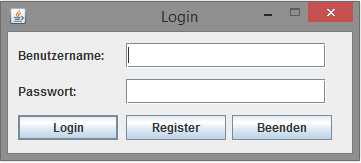
\includegraphics{Bilder/login_client.png}
            \captionof{figure}{wndLogin-Oberfläche}
\end{minipage}

\item wndRegister: Registrations Oberfläche. \\
\begin{minipage}{\linewidth}
            \centering
            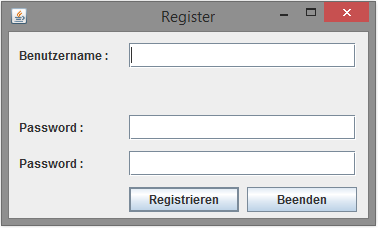
\includegraphics[height=5cm]{Bilder/register_client.png}
            \captionof{figure}{wndRegister-Oberfläche}
\end{minipage}
\end{itemize}

\subsubsection{Utils-Package}
\begin{itemize}
\item CConfigParser: Analog zur gleichnamigen Methode auf dem Server. Liest die config.cfg aus und speichert die darin befindlichen Informationen als Objektattribute des Parsers. Diese können mittels der Getter Methoden ausgelesen werden.
\item CUserErrorMessages: Ist eine Sammlung aller Fehlermeldungen, die dem User ausgegeben werden. Alle Meldungen werden in einem JOptionPane-ConfirmDialog ausgegeben.
\item CUtils: Enthält aktuell nur Methoden, die die Länge auf den Längen-String im Packet parsen. (50 -> 050 bei Nachrichten, 9 -> 09 bei Login-/Registerpackets). Generell soll diese Klasse aber alle sonstigen hilfreichen Methoden umfassen, die irgendwo öfter gebraucht werden könnten.
\end{itemize}
\clearpage

\section{Funktionsweisen und Abläufe}
\subsection{Funktionsweise des Servers}
\begin{figure}[h]
	\centering
	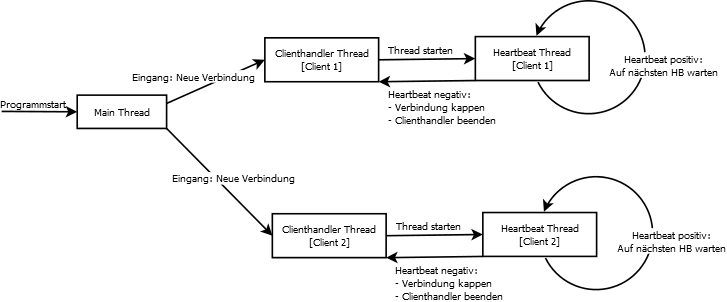
\includegraphics[width=17cm]{Bilder/Serverablauf.png}
	\caption{Funktionsweise des Servers}
\end{figure}
Das Bild zeigt schematisch welche Threads auf dem Server gestartet werden und wie das ganze bei mehreren Clients gehandhabt wird.\\
Zunächst kommt eine neue Verbindung auf dem Server an, daraufhin wird der Clienthandler-Thread (CClientHandler Klasse) erstellt und gestartet. Dieser startet wiederum den Heartbeat Thread für den Client. [Server -> Client] (CHeartbeat)\\
Da aus der Klassenerklärung ersichtlich ist wie der Clienthandler funktioniert, ist dies auf dem Bild ausgelassen.\\
Der Heartbeat funktioniert relativ ein. Es ist eine Schleife, die immer von neuem beginnt zu prüfen ob ein Heartbeat (eine Nachricht o.ä.) angekommen ist. Ist dem so, wird der Thread für 6 Sekunden schlafen gelegt, dann folgt erneut die Überprüfung.\\
Kam kein Packet an dieser Zeit an, so wird die Verbindung gekappt und der Clienthandler beendet. Damit wird auch der Client vom Server abgemeldet.
\clearpage

\subsection{Funktionsweise des Clients}
\begin{figure}[h]
	\centering
	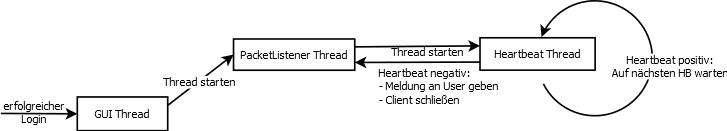
\includegraphics[width=17cm]{Bilder/Clientablauf.png}
	\caption{Funktionsweise des Clients}
\end{figure}
Der Ablauf ist relativ ähnlich zu dem auf dem Server. Bei einem erfolgreichen Login wird ein GUI Thread für die wndChat-Oberfläche gestartet. Diese Oberfläche startet desweiteren einen Packetlistener-Thread (CPacketListener) um eingehende Packete abzufangen und auszuwerten. Diese Thread startet aber wiederum einen weiteren Thread für die Heartbeat Funktion des Clients. [Client -> Server]\\
Die Heartbeat Funktion ist gleich zu der auf dem Server realisiert. Nur dass ausgehende Heartbeat Packets jeweils woanders gesendet werden.
\clearpage

\subsection{Ablauf eines Login}
\begin{figure}[h]
	\centering
	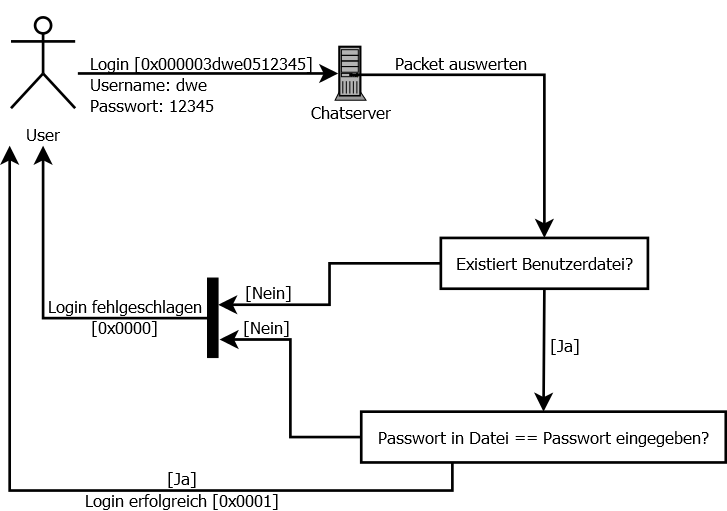
\includegraphics[width=14cm]{Bilder/Ablauf_Login.png}
	\caption{Ablauf eines Login Vorgangs}
\end{figure}
\setlist[enumerate]{itemsep=0cm} 
\begin{enumerate}[label*=\arabic*.]
\item Der Client sendet ein Packet der Form 0x0000XXusernameYYpassword an den Server. XX und YY sind die jeweiligen Längen von username und password.
\item Der Server wertet diese Packet hinsichtlich Form und Inhalt aus. (Stimmt die Form? Stimmen die Längen? Extrahieren von Benutzername und Passwort aus dem Packet)
\item Existiert die zugehörige Benutzerdatei?
\begin{enumerate}[label*=\arabic*.]
      \item Falls ja: Entspricht das angegebene Passwort dem Passwort, das in der Benutzerdatei steht?
      \begin{enumerate}[label*=\arabic*.]
           \item Falls ja: Login erfolgreich Packet 0x0001 an Benutzer zurücksenden.
           \item Falls nein: Login fehlgeschlagen Packet 0x0000 an Benutzer zurücksenden.
\end{enumerate}
      \item Falls nein: Login fehlgeschlagen Packet 0x0000 an Benutzer zurücksenden.
\end{enumerate}
\end{enumerate}
\clearpage
\subsection{Ablauf bei Nachrichten (Serverseitig)}
\begin{figure}[h]
	\centering
	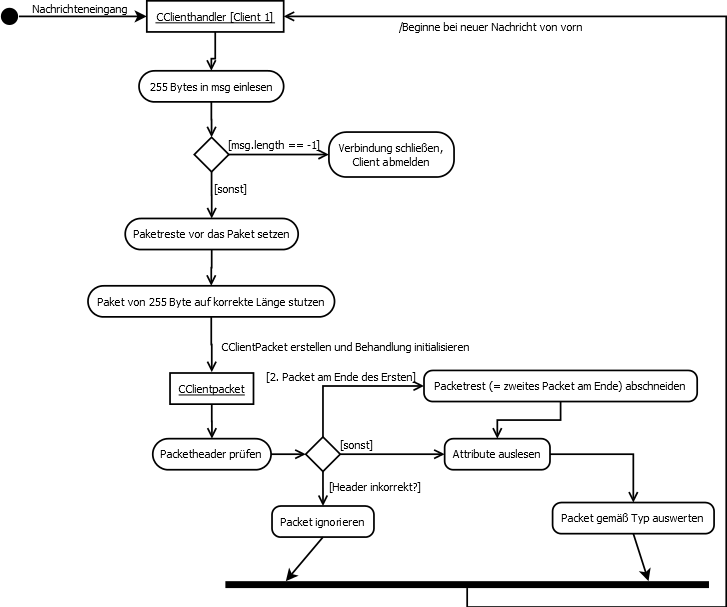
\includegraphics[width=17cm]{Bilder/Ablauf_Nachricht.png}
	\caption{Ablauf einer Nachricht}
\end{figure}
Das Bild ist eigentlich selbsterklärend, deshalb folgt keine weitere Erläuterung des Ablaufs.
\clearpage

\section{Packet Struktur}
Der Server funktioniert mit sogenannten Packets. Das sind Strings, die eine bestimmte Form haben. Sie bestehen im Grunde genommen aus den Teilen \textcolor{blue}{Packetheader} und \textcolor{red}{Packetpayload}. Jedes Packet darf maximal 256 Zeichen lang sein.

Ein Beispielpacket würde wie folgt aussehen: \textbf{0x000003dwe041234}\\
Zerlegt in seine Einzelteile: 0x0000 03 dwe 04 1234\\
\begin{table}[h]
    \centering
    \begin{tabular}{|l|l|}
    \hline
    \textbf{Teil des Packets} & \textbf{Erklärung}                                      \\ \hline
    0x0000           & Packetheader, in diesem Fall Login             \\ \hline
    03               & Länge des ersten Parameters, in diesem Fall 3  \\ \hline
    dwe              & Erster Parameter, in diesem Fall Benutzername  \\ \hline
    04               & Länge des zweiten Parameters, in diesem Fall 4 \\ \hline
    1234             & Zweiter Parameter, in diesem Fall Passwort     \\ \hline
    \end{tabular}
\end{table}

Zusätzlich zu der nachfolgenden Erklärung liegt der Dokumentation eine englische Erklärung der Packetstruktur bei.

\subsection{Packetheader}
Der Packetheader dient als Identifikation des Packets. Er gibt den Typ an, aus dem die weitere Form abzuleiten ist. Nachfolgend eine Liste von Packetheadern, die vom Client zum Server gesendet werden:
\begin{table}[h]
    \centering
    \begin{tabular}{|l|l|}
    \hline
    \textbf{Header} & \textbf{Typ}          \\ \hline
    0x0000 & Login        \\ \hline
    0x0001 & Registration \\ \hline
    0x0002 & Nachricht    \\ \hline
    \end{tabular}
\end{table}

Diese Packetheader können vom Server an den Client gesendet werden:
\begin{table}[h]
    \centering
    \begin{tabular}{|l|l|}
    \hline
    \textbf{Header} & \textbf{Typ}          \\ \hline
    0x0000 & Login abgelehnt          \\ \hline
    0x0001 & Login erfolgreich        \\ \hline
    0x0002 & Registration abgelehnt   \\ \hline
    0x0003 & Registration erfolgreich \\ \hline
    0x0004 & Nachricht                \\ \hline
    \end{tabular}
\end{table}

\subsection{Packetpayload}
Der Payload ist einfach gesagt der Inhalt des Packets. Er teilt sich in Parameter auf. Jedem Parameter wird zudem die eigene Länge vorangesetzt. Die Länge hat immer eine feste Länge, abhängig vom Parametertyp. So haben zum Beispiel die Parameter für Benutzername und Passwort jeweils eine Parameterlänge von 2 Zeichen, Nachrichten hingegen 3 Zeichen. Das hängt damit zusammen, dass bei Nachrichten deutlich mehr Zeichen (bis zu 247 Zeichen) übertragen werden müssen.

Nachfolgend eine Liste mit Packetheadern, der zugehörigen Parameteranzahl und den Parametern inkl. deren Parameterlänge in Klammer (Client -> Server):
\begin{table}[h]
    \centering
    \begin{tabular}{|l|c|l|}
    \hline
    \textbf{Packetheader}          & \textbf{Parameteranzahl} & \textbf{Parameter}                      \\ \hline
    0x0000 (Login)        & 2               & Benutzername [2], Passwort [2] \\ \hline
    0x0001 (Registration) & 2               & Benutzername [2], Passwort [2] \\ \hline
    0x0002 (Nachricht)    & 1               & Nachricht [3]                  \\ \hline
    \end{tabular}
\end{table}

Nachfolgende die gleiche Liste, nur vom Server zum Client.
\begin{table}[h]
    \centering
    \begin{tabular}{|l|c|l|}
    \hline
    \textbf{Packetheader}          & \textbf{Parameteranzahl} & \textbf{Parameter}                      \\ \hline
    0x0000 (Login erfolgreich)           & 0               & ~                         \\ \hline
    0x0001 (Login fehlgeschlagen)        & 0               & ~                         \\ \hline
    0x0002 (Registration erfolgreich)    & 0               & ~                         \\ \hline
    0x0003 (Registration fehlgeschlagen) & 0               & ~                         \\ \hline
    0x0004 (Nachricht)                   & 2               & Sender [2], Nachricht [3] \\ \hline
    \end{tabular}
\end{table}
\end{document}
%-------------------
%Hier endet der Text deiner Hausarbeit
%-------------------